\documentclass[12pt,a4paper]{report}

% --- Paquets bàsics ---
\usepackage[catalan]{babel}
\usepackage[utf8]{inputenc}
\usepackage[T1]{fontenc}
\usepackage{lmodern}
\usepackage{geometry}
\usepackage{setspace}
\usepackage{graphicx}
\usepackage[hidelinks]{hyperref}
\usepackage{amsmath}
\usepackage{amsfonts}
\usepackage{amssymb}
\usepackage{float}
\usepackage{listings}
\usepackage{xcolor}

\lstdefinelanguage{CSharp}{
  language=[Sharp]C
}

\lstset{
  basicstyle=\ttfamily\footnotesize,
  breaklines=true,
  breakatwhitespace=false,
  postbreak=\mbox{\textcolor{red}{$\hookrightarrow$}\space},
  captionpos=b,
  frame=single,
  framerule=0.5pt,
  rulecolor=\color{gray!60},
  aboveskip=6pt,
  belowskip=6pt,
  keywordstyle=\color{blue},
  commentstyle=\color{gray},
  stringstyle=\color{teal},
  showstringspaces=false,
  tabsize=2
}
\begin{document}

\chapter{Comunicació MQTT entre Unity i el sistema SCADA}

Un dels aspectes fonamentals del projecte és la comunicació entre el procés industrial desenvolupat en Unity i el sistema RapidSCADA. Aquesta comunicació es realitza mitjançant el protocol MQTT, àmpliament utilitzat en entorns industrials i aplicacions IoT per la seva simplicitat i eficiència.

Per a la gestió del sistema de missatgeria s'ha utilitzat un \textbf{broker MQTT Mosquitto} \cite{mosquitto_download}, instal·lat localment a l'entorn de desenvolupament. Aquest broker actua com a intermediari en l'intercanvi de dades entre Unity i SCADA, permetent la comunicació en temps real. El sistema s'ha configurat en mode local (\textit{localhost}) per simplificar el desplegament i facilitar el desenvolupament.

\section{Implementació de MQTT a Unity}

La integració de MQTT a Unity s'ha realitzat mitjançant la llibreria \textit{M2MqttUnity}, que permet establir connexions amb un broker MQTT i gestionar tant la publicació com la subscripció a diferents \textit{topics} \cite{mqtt_unity_guide}.

Aquesta llibreria proporciona una estructura base per a la comunicació, sobre la qual s'ha implementat la lògica específica del projecte, incloent la gestió de missatges i la sincronització amb l'estat del sistema.

La configuració del broker i la implementació de MQTT s'han basat en la documentació oficial de Mosquitto \cite{mosquitto_download}.

\subsubsection{Estructura dins de Unity}

La gestió de la comunicació MQTT s'ha implementat mitjançant un script anomenat \textit{MQTTManager}, que està associat a un \textbf{GameObject buit} \cite{UnityGameObjects} dins de l'escena.

Aquest objecte actua de manera independent de la resta de components del sistema, centralitzant tota la comunicació amb el broker MQTT.

Aquest script disposa d'una referència a un objecte anomenat \textit{PlantController}, que conté tota la lògica de control de la planta (GRAFCET, sensors, actuadors, etc.). D'aquesta manera, el \textit{MQTTManager} no implementa la lògica del sistema, sinó que simplement actua com a pont de comunicació entre Unity i l'exterior.

\subsubsection{Inicialització i connexió amb el broker}

La connexió amb el broker MQTT es realitza dins del mètode \texttt{Start()}, que s'executa una sola vegada en iniciar la simulació:

\begin{lstlisting}[language=CSharp, caption=Inicialització de la connexió MQTT]
client = new MqttClient("127.0.0.1");
client.MqttMsgPublishReceived += OnMessageReceived;
client.Connect("UnityClient");

client.Subscribe(
    new string[] { "plant/cmd/#" },
    new byte[] { MqttMsgBase.QOS_LEVEL_AT_LEAST_ONCE }
);
\end{lstlisting}

Cada una d'aquestes línies té una funció específica \cite{mqtt_unity_guide}:

\begin{itemize}
    \item \texttt{new MqttClient("127.0.0.1")} crea el client MQTT i estableix la direcció del broker (en aquest cas, local).
    
    \item \texttt{MqttMsgPublishReceived += OnMessageReceived} associa una funció que s'executarà automàticament cada vegada que arribi un missatge des del broker.
    
    \item \texttt{Connect('UnityClient')} estableix la connexió amb el broker MQTT, identificant el client amb un nom únic.
    
    \item \texttt{Subscribe(...)} permet a Unity subscriure's a tots els topics que comencen per \texttt{plant/cmd}, és a dir, totes les comandes enviades des del sistema extern.
\end{itemize}

Aquesta configuració defineix el comportament principal de Unity dins del sistema MQTT: \textbf{Unity rep comandes i publica dades}.

\subsubsection{Execució contínua de la publicació}

La publicació de dades es realitza dins del mètode \texttt{Update()}, que s'executa en cada fotograma del motor gràfic:

\begin{lstlisting}[language=CSharp]
void Update()
{
    PublishSensors();
    PublishActuators();
    PublishCounters();
    PublishStatus();
}
\end{lstlisting}

Aquesta decisió de disseny permet que el sistema comprovi constantment si hi ha canvis en les variables de la planta. No obstant això, per evitar un excés de missatges MQTT, no es publiquen tots els valors en cada iteració, sinó només aquells que han canviat.

\subsubsection{Optimització amb diccionaris}

Per gestionar aquesta optimització, s'ha utilitzat una estructura de dades de tipus \textbf{diccionari}:

\begin{lstlisting}[language=CSharp]
using System.Collections.Generic;
Dictionary<string, int> lastValues;
\end{lstlisting}

Un diccionari permet emmagatzemar parelles \textit{clau-valor}, on:
\begin{itemize}
    \item La clau és el \textit{topic MQTT}
    \item El valor és l'últim valor enviat
\end{itemize}

Cal destacar que per poder utilitzar aquesta estructura dins de Unity ha estat necessari importar explícitament el \textbf{namespace} \texttt{System.Collections.Generic} \cite{dotnet_collections}. Tot i que forma part de la llibreria estàndard de C\#, en alguns entorns de Unity no està disponible per defecte en l'script si no s'inclou manualment.

Sense aquesta importació, el sistema no reconeix el tipus \texttt{Dictionary}, provocant errors de compilació. Per aquest motiu, és imprescindible afegir aquesta línia a l'inici de l'script per poder utilitzar estructures de dades dinàmiques com els diccionaris.
Això permet comparar el valor actual amb l'últim valor publicat i decidir si és necessari enviar un nou missatge.

\subsubsection{Publicació condicionada}

La funció encarregada d'aquesta lògica és la següent:

\begin{lstlisting}[language=CSharp, caption=Publicació optimitzada]
void PublishIfChanged(string topic, int val){
  if (!lastValues.ContainsKey(topic) || lastValues[topic] != val)
  {
    lastValues[topic] = val;
    client.Publish(topic, Encoding.UTF8.GetBytes(val.ToString()));
  }
}
\end{lstlisting}

El funcionament és el següent:

\begin{itemize}
    \item Si el topic no existeix al diccionari, es publica el valor
    \item Si existeix però el valor ha canviat, també es publica
    \item Si el valor és el mateix, no s'envia cap missatge
\end{itemize}

Per tal d'enviar dades mitjançant MQTT, és necessari convertir els valors a un format compatible amb el protocol. En aquest cas, la llibreria MQTT utilitza dades en format binari (\textit{byte array}). Per aquest motiu, s'utilitza el \textit{namespace} \texttt{System.Text}, que proporciona funcionalitats per a la codificació de text.

Concretament, s'utilitza la classe \texttt{Encoding.UTF8} per convertir un valor numèric a una cadena de text i posteriorment a un array de bytes:

\begin{lstlisting}[language=CSharp]
client.Publish(topic, Encoding.UTF8.GetBytes(value.ToString()));
\end{lstlisting}

Aquest procés es divideix en dues etapes:
\begin{itemize}
    \item Conversió del valor a text mitjançant \texttt{ToString()}
    \item Codificació del text a bytes utilitzant UTF-8
\end{itemize}

\subsubsection{Organització de la informació}

Les dades del sistema es divideixen en quatre grans grups:

\begin{itemize}
    \item \textbf{Sensors}: informació de l'estat de la planta
    \item \textbf{Actuadors}: estat dels elements de moviment
    \item \textbf{Comptadors}: nombre de peces processades
    \item \textbf{Estats}: altres variables d'estat com el mode de funcionament o l'estat de la planta
\end{itemize}

Cada grup es publica en un conjunt de topics estructurats jeràrquicament, per exemple:

\begin{lstlisting}[language=CSharp]
PublishIfChanged("plant/sensors/S1", ...);
PublishIfChanged("plant/actuators/M1", ...);
PublishIfChanged("plant/counters/C1", ...);
\end{lstlisting}

Aquesta estructura facilita la integració amb el sistema SCADA.

\subsubsection{Conversió de dades}

En alguns casos, és necessari transformar dades més complexes en valors simples. Per exemple, el sensor òptic detecta tipus de peça, però MQTT només envia valors numèrics:

\begin{lstlisting}[language=CSharp]
switch (plant.S2.detectedShape)
{
    case PieceShape.Square: shapeValue = 1; break;
    case PieceShape.Cylinder: shapeValue = 2; break;
    case PieceShape.Triangle: shapeValue = 3; break;
}
\end{lstlisting}

Aquesta conversió permet representar informació qualitativa de forma compatible amb el sistema SCADA. En la part de status trobem el següent bloc:
\begin{lstlisting}[language=CSharp]
int emergency = (plant.ETAPA_600 == 600) ? 0 : 1;
PublishIfChanged("plant/alarms/emergency_active", emergency);
int status = 0;
switch (plant.ETAPA_500){
    case 500: status = 0; break; // STOPPED
    case 501: status = 1; break; // AUTO RUNNING
    case 502: status = 1; break; // AUTO STOPPING
    case 503: status = 2; break; // MANUAL RUNNING
    case 504: status = 2; break; // MANUAL STOPPING
}
PublishIfChanged("plant/status/actuation_mode", status);
\end{lstlisting}
 
Aquesta codificacó permet representar el mode del sistema de forma simple, d'igual manera que l'estat d'emergència i l'estat del sistema, facilitant la seva interpretació des del sistema SCADA seguint les etapes que hi hagi actives en el procès d'automatització.

\subsubsection{Recepció de comandes}

Finalment, Unity és capaç de rebre comandes externes mitjançant la funció associada als missatges entrants:

\begin{lstlisting}[language=CSharp, caption=Gestió de comandes]
void OnMessageReceived(object sender, MqttMsgPublishEventArgs e)
{
    string topic = e.Topic;
    int value = int.Parse(Encoding.UTF8.GetString(e.Message));

    if (topic == "plant/cmd/start") plant.B_Start = true;
    if (topic == "plant/cmd/manual/M1") plant.CMD_M1 = value;
}
\end{lstlisting}

Aquest sistema permet modificar el comportament de la planta en temps real des d'un sistema extern.

\subsubsection{Funcionament global}

Seguint la lògica definida en el sistema:

\begin{itemize}
    \item \textbf{Unity publica} tota la informació de la planta (sensors, actuadors i comptadors)
    \item \textbf{Unity es subscriu} als topics de comandes (\texttt{plant/cmd})
\end{itemize}


\section{Implementació de MQTT a RapidSCADA}

De manera paral·lela a Unity, el sistema RapidSCADA també s'ha configurat per utilitzar el protocol MQTT com a mecanisme de comunicació \cite{RapidScadaVideos}. En aquest cas, RapidSCADA actua com a client MQTT, subscrivint-se als \textit{topics} publicats per Unity i publicant les seves pròpies ordres de control.

Així doncs, es defineix una arquitectura complementària a la descrita anteriorment:
\begin{itemize}
    \item RapidSCADA es subscriu als \textit{topics} de dades (sensors, actuadors i comptadors)
    \item RapidSCADA publica als \textit{topics} de comandes (\texttt{plant/cmd})
\end{itemize}

Aquesta distribució de rols segueix el model típic dels sistemes industrials, on el SCADA supervisa i envia ordres al sistema de control.

\subsubsection{Configuració de la comunicació MQTT}

Un dels avantatges de RapidSCADA és que ja incorpora suport natiu per MQTT, per la qual cosa no és necessari instal·lar cap plugin extern addicional.

La configuració es realitza des del mòdul \textit{Communicator} \cite{rapidscada_device_polling}, seguint els passos següents:

\begin{enumerate}
    \item Crear una nova línia de comunicació dins de l'apartat \textit{Communication Lines}.
    
    \item Seleccionar el protocol MQTT, concretament el tipus \textbf{MQTT Client}.
    
    \item Configurar els paràmetres de connexió. En aquest projecte s'han mantingut els valors per defecte:
    \begin{itemize}
        \item \textbf{Servidor}: \textit{localhost}
        \item \textbf{Port}: 1883
    \end{itemize}
    
\end{enumerate}

Aquesta configuració permet establir la connexió amb el mateix broker local utilitzat per Unity.

\begin{figure}[H]
    \centering
    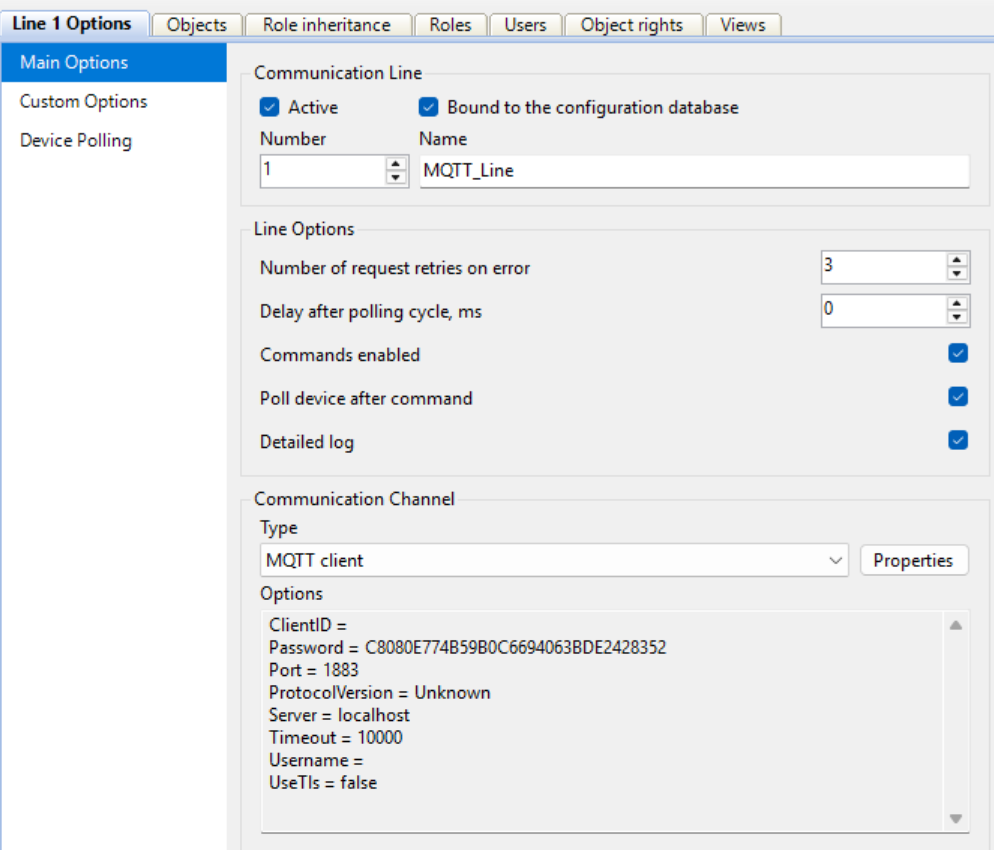
\includegraphics[width=0.45\linewidth]{images/comm_line_mqtt.png}
    \caption{Creació \textit{Communication Line} en RapidScada}
\end{figure}
\subsubsection{Configuració del dispositiu MQTT}

Un cop definida la línia de comunicació, el següent pas és crear un dispositiu associat a aquesta línia.

Dins d'aquest dispositiu, cal configurar el driver:
\begin{itemize}
    \item \textbf{Driver}: \texttt{DrvMqttClient}
\end{itemize}

Aquest driver és l'encarregat de gestionar la comunicació MQTT dins de RapidSCADA.

\begin{figure}[H]
    \centering
    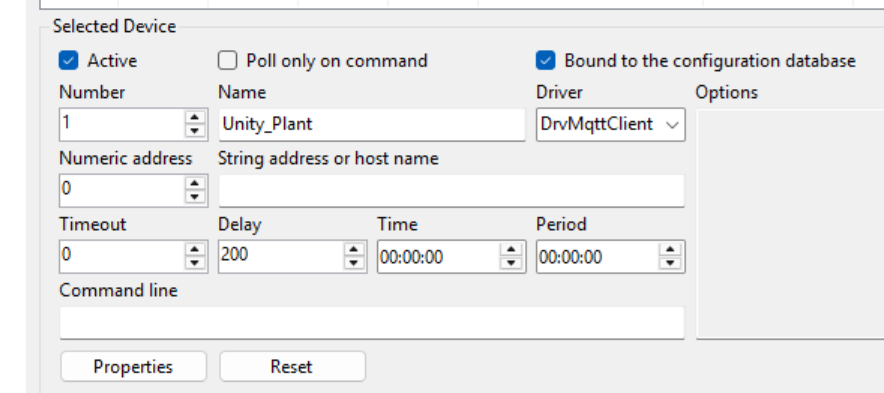
\includegraphics[width=0.5\linewidth]{images/device_mqtt.png}
    \caption{Creació \textit{Device} en RapidScada}
\end{figure}

En aquesta etapa es defineixen dos elements fonamentals:

\paragraph{Subscripcions (\textit{Subscriptions})}

Permeten especificar els \textit{topics} als quals RapidSCADA es subscriurà per rebre dades des de Unity.

Per a cada subscripció es defineix:
\begin{itemize}
    \item El \textbf{topic MQTT}
    \item Un \textbf{identificador o tag}
    \item El tipus d'accés (normalment només lectura)
    \item Opcionalment, un codi en JavaScript per processar les dades rebudes
\end{itemize}

En aquest projecte, no s'ha utilitzat processament addicional, ja que cada variable es publica en un \textit{topic} independent, facilitant el seu tractament directe.

És important destacar que, tot i que una subscripció està pensada principalment per a la lectura de dades, en el context de Rapid SCADA el canal associat pot utilitzar-se tant com a \textit{input channel} com a \textit{output channel}. Això permet que un mateix \textit{topic} pugui servir tant per rebre com per enviar valors, depenent de la configuració del canal.

\paragraph{Comandes (\textit{Commands})}

Permeten definir els \textit{topics} als quals RapidSCADA enviarà informació.

Aquests \textit{topics} corresponen a les ordres que controlen el comportament de la planta en Unity, com per exemple ordres manuals o canvis de mode de funcionament.


A diferència de les subscripcions, els \textit{topics} definits com a comandes tenen un comportament exclusivament d'escriptura. Això implica que només s'utilitzen per enviar dades i no permeten la lectura del seu valor des de Rapid SCADA a través del mateix canal.

Aquest comportament segueix la lògica pròpia del protocol MQTT, on per rebre dades és necessari estar subscrit a un \textit{topic}, mentre que per enviar dades només cal publicar-hi informació, sense necessitat de subscripció prèvia.

\begin{figure}[H]
\centering
\begin{minipage}{0.42\textwidth}
    \centering
    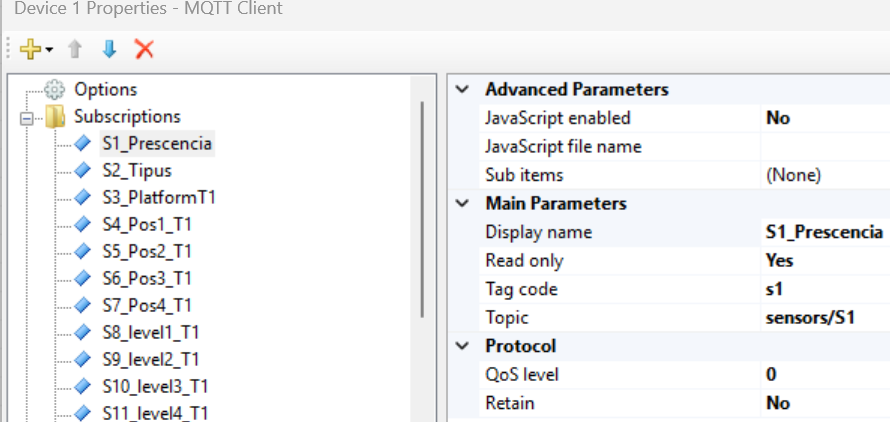
\includegraphics[width=\linewidth]{images/subscription.png}
\end{minipage}
\hfill
\begin{minipage}{0.52\textwidth}
    \centering
    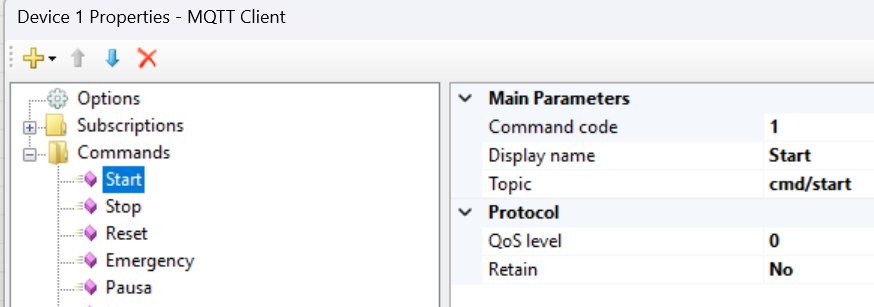
\includegraphics[width=\linewidth]{images/commands.png}
\end{minipage}
\caption{\textit{Subscriptions} i \textit{Commands} en RapidScada}
\end{figure}

\subsubsection{Creació dels canals}

Una vegada configurat el dispositiu, és necessari crear els canals (\textit{channels}) \cite{rapidscada_channels} que representaran cadascuna de les variables dins del sistema SCADA.

Per a cada canal es defineix:
\begin{itemize}
    \item La línia de comunicació associada
    \item El dispositiu MQTT
    \item L'objecte (habitualment \textit{Enterprise})
    \item El valor o índex del canal corresponent
\end{itemize}

Aquests canals actuen com a punt d'accés a les dades dins del sistema.

\subsubsection{Configuració avançada dels canals}

Finalment, tots els canals creats es poden visualitzar i configurar des de la base de dades de configuració, concretament a la taula \textit{Channels} dins de \textit{Primary Table}.

En aquesta taula es poden ajustar diversos paràmetres:

\begin{itemize}
    \item Tipus d'accés (lectura o escriptura)
    \item Tipus de dada (per exemple: \textit{On-Off}, \textit{Yes-No})
    \item Nombre de decimals
    \item Altres propietats de visualització
\end{itemize}

Cal destacar que, en alguns casos, hauria estat útil treballar amb variables de tipus \textit{string}. No obstant això, no s'ha aconseguit visualitzar correctament aquest tipus de dades dins de RapidSCADA en el context del projecte.

\section{Funcionament global}

Amb tota la configuració completada, el funcionament del sistema és el següent:

\begin{itemize}
    \item RapidSCADA rep en temps real totes les dades publicades per Unity
    \item RapidSCADA permet supervisar l'estat de la planta
    \item RapidSCADA envia ordres a Unity mitjançant els \textit{topics} de comanda
\end{itemize}

Aquesta comunicació bidireccional permet implementar un sistema SCADA complet, amb capacitat tant de monitoratge com de control sobre el procés industrial simulat.
\end{document}

https://www.emqx.com/en/blog/using-mqtt-in-unity-with-m2mqttunity-library-a-step-by-step-guide


https://www.youtube.com/playlist?list=PLeyJvzEKXs5D6zYUfeV52KXy479tg0w9U
b

https://learn.microsoft.com/en-us/dotnet/api/system.collections.generic?redirectedfrom=MSDN&view=net-7.0

https://learn.microsoft.com/es-es/dotnet/api/system.text?view=net-8.0


@misc{mosquitto_download,
  title = {Eclipse Mosquitto Download},
  howpublished = {\url{https://mosquitto.org/download/}}
}

@misc{m2mqttunity_guide,
  title = {Using MQTT in Unity with M2MqttUnity},
  howpublished = {\url{https://www.emqx.com/en/blog/using-mqtt-in-unity-with-m2mqttunity-library-a-step-by-step-guide}}
}